\documentclass[11pt,a4paper,twoside,french,svgnames]{report}
\usepackage[utf8]{inputenc} % force the use of utf8
\usepackage[T1]{fontenc} % font encoding, allows accents
\usepackage[papersize={21cm,29.7cm},top= 2.5cm,bottom=2.5cm, inner=2.5cm, outer=2.5cm]{geometry} % page formatting
\usepackage[francais]{babel} % translate everything in the desired language: table of contents, etc. 'english' can be replaced with 'francais'
\usepackage{graphicx} % images management
\usepackage{wrapfig} % floating images
\usepackage{array} % allow arrays
\usepackage{fancyhdr} % headers/footers management (overrides empty, plain and headings)
\usepackage{listings} % code insertion (MUST BE WRITTEN AFTER BABEL)
%\usepackage[nottoc,numbib]{tocbibind} % bib in toc
%\usepackage{pdfpages} % include PDF documents
\usepackage{enumitem} % for /setlist
\usepackage{color,soul} % add some colors and hightlight
\usepackage{xcolor} % more colors
\usepackage[hyphens]{url} % auto break lines in URL
\usepackage[hidelinks,  colorlinks  = true, % no borders, colors enabled
                        anchorcolor = blue,
                        linkcolor   = black, % links in table of contents
                        urlcolor    = blue,
                        citecolor   = blue]{hyperref}
%\usepackage[%nonumberlist,% no page number
%            toc,% displayed in toc
%            numberedsection,% displayed as a numbered section in toc
%            xindy]{glossaries} % glossary with xindy style. MUST BE WRITTEN AFTER HYPERREF
%\setglossarystyle{listgroup}

\sethlcolor{cyan} % package soul
\newcommand{\file}[1]{\hl{\emph{#1}}} % highlight a file URI

%\makeglossaries
%\loadglsentries{glossary.tex}

%%%%%%%%%%%%%%%%%%%%%%%%%%%%%%%%%%%%%%%%%%%%%%%%%%%%%%%% LISTINGS %%%%%%%%%%%%%%%%%%%%%%%%%%%%%%%%%%%%%%%%%%%%%%%%%%%%%%%%
\definecolor{comment}{rgb}{0.12, 0.38, 0.18 } % adjusted, in Eclipse: {0.25, 0.42, 0.30 } = #3F6A4D
\definecolor{keyword}{rgb}{0.37, 0.08, 0.25}  % #5F1441
\definecolor{string}{rgb}{0.06, 0.10, 0.98} % #101AF9

\lstset{
  columns=flexible, %prevent extra spaces
  rulecolor=\color{black!50},
  backgroundcolor = \color{blue!10},
  numbers=none, % line numbering
  showspaces=false,
  showtabs=false,
  breaklines=true,
  showstringspaces=false,
  breakatwhitespace=false,
  commentstyle=\color{comment},
  keywordstyle=\color{keyword},
  stringstyle=\color{string},
  basicstyle=\ttfamily,
  extendedchars=true,
  emph=[2]{In},
  emphstyle=[2]\color{black!70},
  morecomment=[l][\color{blue}]{Out},
  frame=single,
  frameround=tttt,
  framerule=0.3pt,
  framesep=4pt,
  belowcaptionskip=2.1pt,
  literate={à}{{\`a}}1 {â}{{\^a}}1 %                         letter a
           {À}{{\`A}}1 {Â}{{\^A}}1 %                         letter A
           {ç}{{\c{c}}}1 %                                   letter c
           {Ç}{{\c{C}}}1 %                                   letter C
           {é}{{\'e}}1 {è}{{\`e}}1 {ê}{{\^e}}1 {ë}{{\"e}}1 % letter e
           {É}{{\'E}}1 {È}{{\`E}}1 {Ê}{{\^E}}1 {Ë}{{\"E}}1 % letter E
           {î}{{\^i}}1 {ï}{{\"i}}1 %                         letter i
           {Î}{{\^I}}1 {Ï}{{\"I}}1 %                         letter I
           {ô}{{\^o}}1 %                                     letter o
           {Ô}{{\^O}}1 %                                     letter O
           {œ}{{\oe}}1 %                                     letter oe
           {Œ}{{\OE}}1 %                                     letter OE
           {ù}{{\`u}}1 {û}{{\^u}}1 {ü}{{\"u}}1 %             letter u
           {Ù}{{\`U}}1 {Û}{{\^U}}1 {Ü}{{\"U}}1 %             letter U
  % above is a hack to force UTF8 compatibility (only for french)
}

\newcommand{\textcode}[1]{\lstset{
  language=,
  title={{\setlength{\fboxsep}{1pt}\fcolorbox{orange}{yellow!20}{\sffamily\scriptsize
              \textcolor{gray!10}{\_}{#1}\textcolor{gray!10}{\_}}}}
  }
}

\newcommand{\vhdl}{\lstset{
  language=VHDL,
  title={{\setlength{\fboxsep}{1pt}\fcolorbox{orange}{yellow!20}{\sffamily\scriptsize
              \textcolor{gray!10}{\_}VHDL\textcolor{gray!10}{\_}}}}
  }
}
%%%%%%%%%%%%%%%%%%%%%%%%%%%%%%%%%%%%%%%%%%%%%%%%%%%%%%%%%%%%%%%%%%%%%%%%%%%%%%%%%%%%%%%%%%%%%%%%%%%%%%%%%%%%%%%%%%%%%%%%%%%

%\parindent=20pt
\fancypagestyle{plain}{
    % Headers
    \fancyhead[R]{Rapport TP2 MI01}
    \fancyhead[L]{Romain \textsc{PELLERIN} - Kyâne \textsc{PICHOU}}

    % Footers
    \renewcommand{\footrulewidth}{0.1pt}
    \fancyfoot[C]{Université de Technologie de Compiègne}
    \fancyfoot[LE]{\ifnum\thepage>0 \thepage \fi}
    \fancyfoot[RO]{\ifnum\thepage>0 \thepage \fi}
}

\fancypagestyle{empty}{%
    \renewcommand{\headrulewidth}{0pt} % No sub line
    \fancyhead{} % Empty the header

    \renewcommand{\footrulewidth}{0pt}
    \fancyfoot{}
} 

\setlist[itemize,2]{label={$\bullet$}} % use bullets for nested itemize

% First page
\newcommand{\presentation}[1]{\vspace{0.3cm}\large{\textbf{#1}}\vspace{0.3cm}\\}
\newcommand{\presentationLarge}[1]{\vspace{0.3cm}\LARGE{\textbf{#1}}\vspace{0.3cm}\\}

% Overrides chapter (numbered and no-numbered) headings: remove space, display only the title
\makeatletter
  \def\@makechapterhead#1{%
  \vspace*{0\p@}% avant 50
  {\parindent \z@ \raggedright \normalfont
    %\ifnum \c@secnumdepth >\m@ne
    %    \huge\bfseries \@chapapp\space \thechapter
    %    \par\nobreak
    %    \vskip 20\p@
    %\fi
    \interlinepenalty\@M
    \Huge \bfseries \thechapter\quad #1   
    \vskip 40\p@
  }}
  \def\@makeschapterhead#1{%
  \vspace*{0\p@}% before 50
  {\parindent \z@ \raggedright
    \normalfont
    \interlinepenalty\@M
    \Huge \bfseries  #1\par\nobreak
    \vskip 40\p@
  }}
\makeatother

\newcommand{\ignore}[1]{} % inline comments

\pagenumbering{arabic}
%\addtocounter{page}{-7} % page numbering starts at 1 + (-7)
\pagestyle{plain} % uses fancy

\title{Rapport MI01}
\author{Romain PELLERIN et Kyâne PICHOU}
\date\today

%\setcounter{tocdepth}{4}

\begin{document}
\thispagestyle{empty} % only for the current page

\begin{center}

\includegraphics[height=3cm]{UTC_logo.png}\\
\vspace{2.5cm}
\presentation{Université de Technologie de Compiègne} 
\presentation{MI01}

\vspace{2cm}
\noindent\fbox{
\begin{minipage}{0.9\textwidth}
\begin{center}
    \presentationLarge{Rapport de TP}
    \presentationLarge{\Huge{2 - VHDL Séquentiel}}
\end{center}
\end{minipage}}
\vspace{3cm}

\presentation{Automne 2014}
\vspace{1cm}

\def\arraystretch{1.5} % 1 is the default
\begin{tabular}{|>{\hfill\arraybackslash}p{5cm}|p{5cm}|}
\hline
    \multicolumn{2}{|c|}{Romain \textsc{PELLERIN} - Kyâne \textsc{PICHOU}}\\
\hline
     \multicolumn{2}{|c|}{Groupe 1}\\% dates
\hline
    \multicolumn{2}{|c|}{\textit{\today}}\\% dates
\hline
\end{tabular}
\end{center}

\tableofcontents

\chapter{Introduction}
\section{Résumé}
L'objectif de ce TP est d'écrire un programme permettant la gestion d'une ludothèque composée de jeux de société. Un jeu de société est décrit par une fiche contenant les informations suivantes :
\begin{itemize}
  \item Nom du jeu
  \item Genre du jeu : PLATEAU, RPG, COOPERATIF, AMBIANCE ou HASARD
  \item Le nombre de joueurs minimum
  \item Le nombre de joueurs maximum
  \item La durée moyenne d'une partie en minutes
\end{itemize}

\section{Structuration du projet}
Nous avons choisi de structuer notre projet en 5 fichiers pour une meilleure clarté, selon les deux entités principales que sont les \textbf{ludothèques} et les \textbf{jeux} :

\begin{itemize}
  \item \textbf{main.c} Le fichier source contenant le programme principal
  \item \textbf{ludotheque.h} Le fichier d'en-tête contenant les déclarations des structures et fonctions d'une ludothèque
  \item \textbf{ludotheque.c} Le fichier source contenant la définition de chaque fonction d'une ludothèque
  \item \textbf{jeu.h} Le fichier d'en-tête contenant les déclarations des structures et fonctions d'un jeu
  \item \textbf{jeu.c} Le fichier source contenant la définition de chaque fonction d'un jeu
\end{itemize}

\section{Code source}
Le code source est fourni dans l'archive ZIP contenant ce rapport.
\chapter{Exercices}
\section{Exercice 1 - Compteur de 2 bits}

Le but de cet exercice est de modéliser un compteur synchrone à 2 bits. Celui-ci utilisera une horloge et un un signal de reset synchrone. Ces deux fonctionnalités seront implémentées respectivement sur \textbf{PB\_0} et \textbf{PB\_1} qui sont des boutons poussoirs. L'affichage de sortie se fera sur \textbf{LED\_10} qui est un ensemble de deux leds.

\medskip

\noindent La modélisation respectera 2 conditions :
\begin{itemize}
  \item Le front montant de l’horloge est le front actif.
  \item Le reset est actif au niveau bas (\textbf{PB\_1 = '1'})
\end{itemize}
Ainsi, à chaque pression sur le bouton poissoir \textbf{PB\_0}, les LEDs afficheront successivement : '00', '01', '10', '11', '00', '01', etc. Si \textbf{PB\_1} est pressé puis \textbf{PB\_0}, le compteur sera réinitialisé à 0.

\subsection{Ports utilisés}

Au préalable, nous avons décommenté les lignes du fichier \textbf{carte\_tp.ucf} correspondant aux ports utilisés :
\textcode{Fichier : carte\_tp.ucf}
\begin{lstlisting}
NET "LED_10<0>"     LOC = "P44"     | IOSTANDARD = LVCMOS33;
NET "LED_10<1>"     LOC = "P51"     | IOSTANDARD = LVCMOS33;
NET "PB_0"          LOC = "P128"    | IOSTANDARD = LVCMOS33 | CLOCK_DEDICATED_ROUTE = FALSE;
NET "PB_1"          LOC = "P141"    | IOSTANDARD = LVCMOS33 | CLOCK_DEDICATED_ROUTE = FALSE;
\end{lstlisting}

\subsection{VHDL}

Nous proposons une modélisation VHDL de type \textbf{comportementale} puisque c'est plus simple à écrire et parfaitement adapté à notre besoin. En effet nous souhaitons utiliser \textbf{PROCESS} (instructions séquentielles). Les \textbf{signaux déclencheurs} du \textbf{PROCESS} seront les deux boutons poussoirs. Les deux LED permettent \og d'afficher\fg{} 4 valeurs décimales :
\begin{itemize}
  \item 0 soit 00 en binaire sur 2 bits
  \item 1 soit 01 en binaire sur 2 bits
  \item 2 soit 10 en binaire sur 2 bits
  \item 3 soit 11 en binaire sur 2 bits
\end{itemize}
Voici l'implémentation :

\textcode{Fichier : tp2\_1.vhd}
\vhdl
\begin{lstlisting}
entity tp2_1 is
  PORT(LED_10 : out integer range 0 to 3; -- la led peut afficher 4 valeurs sur 2 bits
        PB_0 : in bit;
        PB_1 : in bit); 
end tp2_1;

architecture Behavioral of tp2_1 is
begin
	process(PB_0,PB_1)
	variable i : integer range 0 to 3 := 0; -- variable qui sert d'alias du signal
	begin
		if (PB_1 = '1') then
			i := 0; -- dès que PB_1 est enfoncé, on reset
		elsif(PB_0'event AND PB_0='1') then
			i := i + 1; -- on incrémente à chaque pression de PB_0
		end if;
		LED_10 <= i; -- on affecte la valeur de la variable au signal
	end process;
end Behavioral;
\end{lstlisting}

\subsection{Synthèse}

\noindent On synthétise notre circuit :
\begin{figure}[!h]
   \centering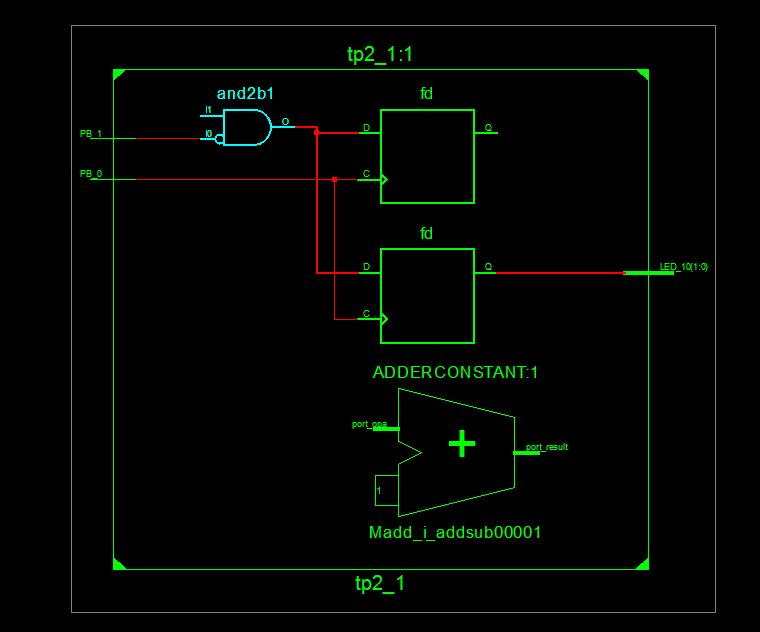
\includegraphics[width=0.95\textwidth]{files/tp2_1/RTL.png}
   \caption{Schéma \og RTL\fg{}}
\end{figure}

On constate que le synthétiseur a utilisé un circuit additionneur avec peu de portes. C'est un circuit \og pré-optimisé\fg{}, indépendant du FPGA cible. C'est une représentation logique du VHDL.

\begin{figure}[!h]
   \centering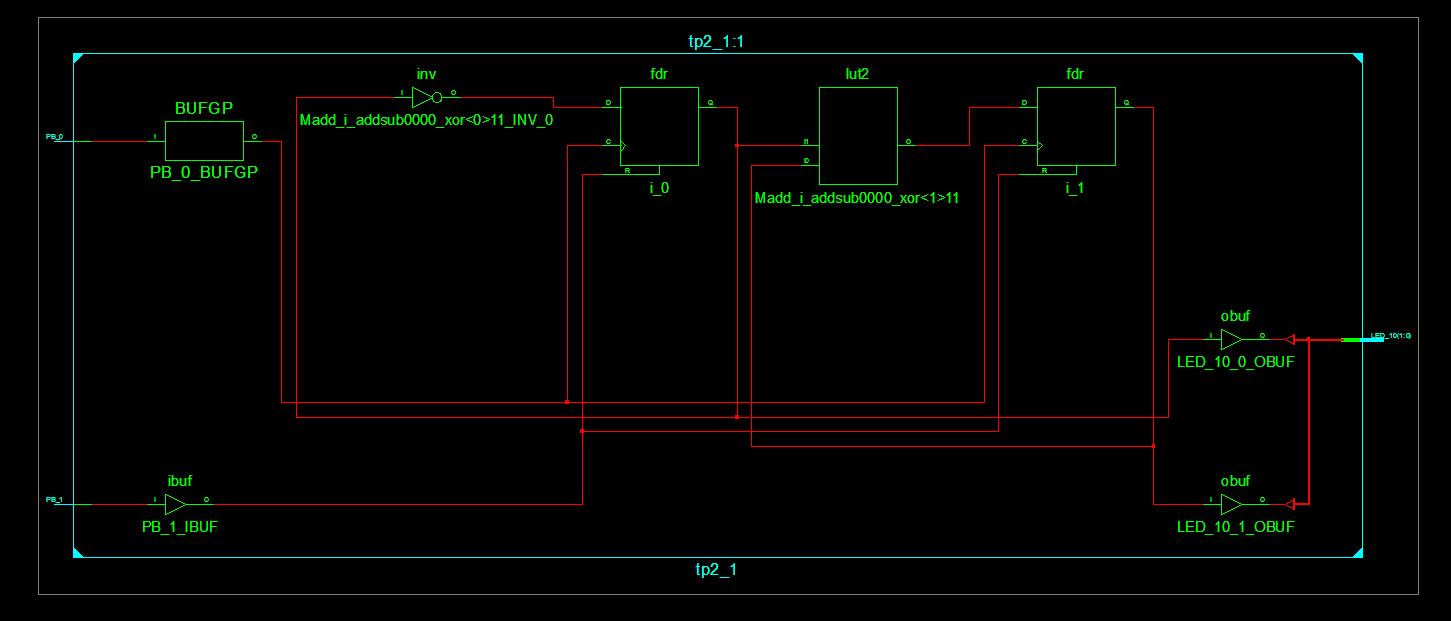
\includegraphics[width=\textwidth]{files/tp2_1/Tech.png}
   \caption{Schéma \og Technology\fg{}}
\end{figure}

Le schéma \og Technology\fg{} présente plus d'éléments que le schéma précédent (\textit{inv}, \textit{fdr}, etc) et est par conséquent beaucoup plus complexe. Ce schéma est généré après l'optimisation, qui est faite en fonction du FPGA cible. Les composants sont choisis selon ce FPGA cible. C'est une représentation technologique du VHDL optimisé.

\subsection{Simulation}

Après la synthèse, on simule notre circuit pour vérifier qu'il respecte le cahier des charges :

\begin{figure}[!h]
   \centering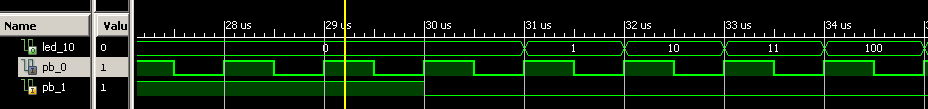
\includegraphics[width=\textwidth]{files/tp2_1/simulateur.png}
   \caption{Simulation}
\end{figure}

La simulation est correcte, nous avons bien un compteur incrémenté suivant l'horloge, qui est réinitialisé par le signal de reset (de façon synchrone avec le signal horloge\footnote{Pour reset notre compteur, il faut que le bouton reset soit actif (\textbf{PB\_1 = '1'}) lors du front d'horloge. En pratique, l'horloge est simulée à l'aide d'un bouton poussoir, de ce fait il fait garder le reset enfoncé (\textbf{PB\_1}) puis appuyer sur le bouton d'horloge (\textbf{PB\_0})}). En effet, au début du schéma, on constate que tant que \textbf{PB\_1} est \og enfoncé\fg{} (équivalent à 1), la valeur des LED est 0. Puis, lorsque le bouton poussoir est relâché (à partir de 30$\mu$s), la valeur affichée par les LED s'incrémente (01, 10, 11, 00, 01, etc).

\bigskip

Pour terminer on programme le FPGA avec notre code pour tester en pratique le bon fonctionnement. Après tests, notre programme est fonctionnel. On constatera que le reset est ici à nouveau synchrone.

\newpage
\section{Exercice 2 - Détecteur de code}
\label{ex2}

Dans cet exercice nous alons modéliser le détecteur de code étudié en TD. Celui-ci lit sur une ligne de transmission série (de 1 bit) par une technique séquentielle synchrone. Un signal \textbf{Alarme} est mis à 1 dès que le code "11010" est détecté. On utilise différents signaux :
\begin{itemize}
\item BP\_0 pour l’horloge (bouton poussoir)
\item SW\_0 pour la ligne de transmission série (switch)
\item LED\_0 pour le signal Alarme
\end{itemize}

\subsection{Ports utilisés}

Au préalable, nous avons décommenté les lignes du fichier \textbf{carte\_tp.ucf} correspondant aux ports utilisés :
\textcode{Fichier : carte\_tp.ucf}
\begin{lstlisting}
NET "LED_0" LOC = "P44"  | IOSTANDARD = LVCMOS33;
NET "SW_0"  LOC = "P130" | IOSTANDARD = LVCMOS33;
NET "PB_0"  LOC = "P128" | IOSTANDARD = LVCMOS33 | CLOCK_DEDICATED_ROUTE = FALSE;
\end{lstlisting}

\subsection{VHDL}

On propose la modélisation VHDL \textbf{comportementale} ci-dessous. Chaque fausse entrée nécessite de re-entrer l'intégralité du code. Il s'agit finalement de modéliser une \textbf{machine à états}.

\vhdl
\begin{lstlisting}
entity tp2_2 is
  port(PB_0,SW_0 : in bit;
       LED_0 : out bit);	
end tp2_2;

architecture Behavioral of tp2_2 is
begin
	process(PB_0) -- Synchronisé sur chaque pression du bouton poussoir
	variable nbt : integer range 0 to 5; -- Un état pour chaque élément du code détecté + l'état où rien n'est détecté
	variable allume : bit := '0'; -- alias du signal de la LED
	begin
	if(PB_0'event and PB_0='1') then
		case nbt is
			-- A chaque pression du bouton poussoir, on vérifie que l'état du switch (1 ou 0) correspond a l'élément du code attendu (selon l'état actuel de la machine), sinon on retombe dans l'état 0 (aucun élément du code détecté)
			when 0 =>
				if(SW_0='1') then
					nbt:=1;
				end if;
			when 1 =>
				if(SW_0='1') then
					nbt:=2;
				else
					nbt:=0;
				end if;
			when 2 =>
				if(SW_0='0') then
					nbt:=3;
				else
					nbt:=0;
				end if;
			when 3 =>
				if (SW_0 ='1') then
					nbt:=4;
				else
					nbt:=0;
				end if;
			when 4 =>
				nbt:=0;
				if(SW_0='0') then -- Le code entier a été détecté
					nbt:=5;
					allume := '1';
				else
					nbt:=0;
				end if;
			when 5 => -- Une fois le code détecté (état = 5), on réinitialise tout peu importe l'état du switch
				nbt:=0;
				allume:='0';
			end case;
			LED_0<=allume; -- Affectation réelle
		end if;
	end process;				
end Behavioral;
\end{lstlisting}

\subsection{Synthèse}

\begin{figure}[!h]
   \centering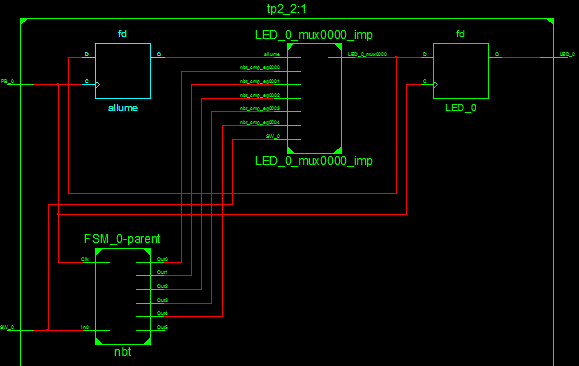
\includegraphics[width=0.74\textwidth]{files/tp2_2/rtl.png}
   \caption{Schéma RTL}
\end{figure}

On remarque que notre état (nbt) est codé sur 5 bits. Pourtant dans notre code VHDL, c'est un entier de 0 à 5, 3 bits auraient donc, à priori, été suffisants.
Au lieu d'utiliser le codage d'un entier en binaire, le synthétiseur utilise 5 bits qui activent où non un multiplexeur. Chaque bit correspond à un état.

\subsection{Simulations}

On simule notre circuit synthétisé dans ISim pour constater son bon fonctionnement.
\begin{figure}[!h]
   \centering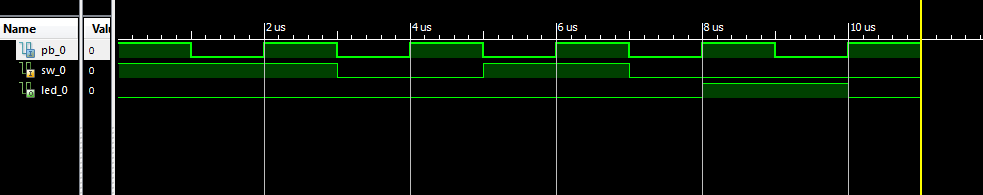
\includegraphics[width=\textwidth]{files/tp2_2/simulateur.png}
   \caption{Simulation}
\end{figure}

On fait évoluer l'entrée d'horloge à une fréquence donnée et on force les valeurs correspondant à notre code sur l'entrée ligne. On constate bien que, dès que le code est détecté, la LED s'allume (passage à 1). Elle repasse à 0 au coup d'horloge suivant, prête à détecter à nouveau le code.

\medskip

On effectue une seconde simulation pour \textbf{vérifier que lorsqu'il y a une mauvaise entrée, il y a bien réinitialisation de la machine à état}. Pour cela on compose le code avec une erreur au milieu. Si le code n'est pas détecté, c'est que l'erreur a bien été prise en compte :
\begin{figure}[!h]
   \centering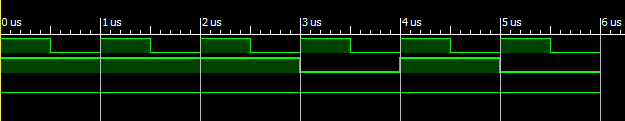
\includegraphics[width=\textwidth]{files/tp2_2/simu_erreur.png}
   \caption{Simulation}
\end{figure}

Ici, le code est correct à l'exception du 3ème '1' (à 2 $\mu$s) qui vient se glisser pour créer une erreur. On remarque que le code n'est donc pas détecté.

\bigskip

Après programmation du FPGA, on constate le bon fonctionnement pratique de notre système.

\newpage
\section{Exercice 3 - Détecteur de code - Fausse entrée négligée}

Il s'agit de répéter l'exercice 2 (section \ref{ex2}) mais en négligeant les fausses entrées.

\subsection{VHDL}

On propose la modélisation VHDL \textbf{comportementale} ci-dessous. Chaque fausse entrée est négligée. Il s'agit à nouveau de modéliser une \textbf{machine à états}.

\vhdl
\begin{lstlisting}
entity tp2_3 is
  port(PB_0,SW_0 : in bit;
       LED_0 : out bit);  
end tp2_3;

architecture Behavioral of tp2_3 is
begin
  process(PB_0)
  variable nbt : integer range 0 to 5;
  variable allume : bit := '0';
  begin
  if(PB_0'event and PB_0='1') then
    case nbt is
      when 0 =>
        if(SW_0='1') then
          nbt:=1;
        end if;
      when 1 =>
        if(SW_0='1') then
          nbt:=2;
        end if;
      when 2 =>
        if(SW_0='0') then
          nbt:=3;
        end if;
      when 3 =>
        if (SW_0 ='1') then
          nbt:=4;
        end if;
      when 4 =>
        nbt:=0;
        if(SW_0='0') then
          nbt:=5;
          allume := '1';
        end if;
      when 5 =>
        nbt:=0;
        allume:='0';
      end case;
      LED_0<=allume;
    end if;
  end process;        
end Behavioral;
\end{lstlisting}

Le code proposé ci-dessus permet d'ignorer les fausses entrées. Lorsqu'il y a une erreur elle n'est pas prise en compte et la machine à états reste inchangée.

\subsection{Synthèse}

\begin{figure}[!h]
   \centering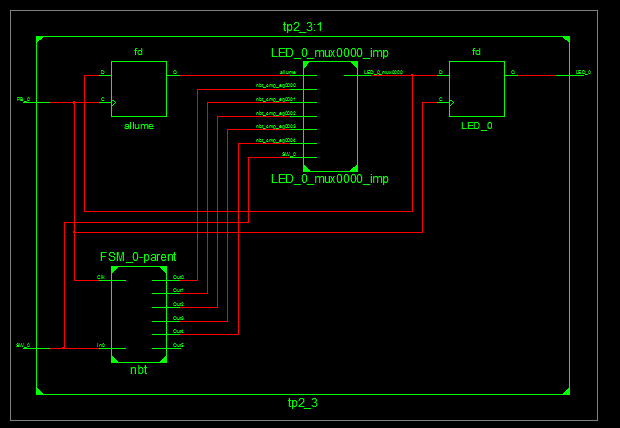
\includegraphics[width=0.74\textwidth]{files/tp2_3/rtl.png}
   \caption{Schéma RTL}
\end{figure}

\noindent Le nombre de bits d'état est étrangement le même que dans l'exercice 2.

\subsection{Différences par rapport à l'exercice 2}

On simule notre code à la même manière que dans l'exercice 2. On entre le bon code mais on glisse une erreur au milieu. Cette fois-ci l'erreur ne devrait pas être prise en compte et le code devrait être détecté :
\begin{figure}[!h]
   \centering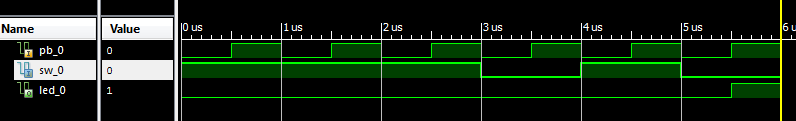
\includegraphics[width=\textwidth]{files/tp2_3/simu_erreur.png}
   \caption{Simulation}
\end{figure}

Notre simulation est concluante. Le troisième '1' était une erreur mais le code a tout de même été détecté. La fausse entrée a donc été négligée.
%\chapter{Conclusion générale}

\section{OpenGL ou Unity}

La plus grosse problématique du projet aura été le choix entre Unity et OpenGL. Nous étions initalement partis sur du développement en OpenGL mais heureusement, en début d'année 2015, Unity a rendu son moteur totalement gratuit, nous permettant ainsi de pouvoir l'utiliser. Nous nous en sommes rendus compte peu de temps après le début du projet et avons ainsi changé de technologie. Nous avons tout de même eu le temps d'essayer OpenGL et il s'était avéré que le développement aurait été bien trop dur et presque impossible. Effectivement, nous ne connaissions pas cette technologie et la contrainte de temps (un semestre) ne nous aurait pas permis de l'appréhender.

\section{Problèmes}

Un autre problème aura été l'utilisation du SDK de Google. Au départ nous ne savions pas comment faire déplacer le joueur, nous étions donc partis sur l'utilisation d'une \textit{library} tierce, Dive. Or il s'est avéré que cette \textit{library} souffrait d'un bug au niveau du gyroscope. Nous avons finalalement réussi à utiliser uniquement le SDK de Google et faire avancer notre joueur.

\section{Jeu final et objectifs}

Au final, un seul de nos objectifs complémentaires a été atteint : rajouter une ambiance sonore (une musique de fond). Nous sommes néanmoins très satisfaits du résultat visuel et du jeu de manière générale. Avoir plus de temps nous aurait probablement permis d'atteindre d'autres objectifs.

\end{document}
